\documentclass[letterpaper,12pt]{article}

\usepackage{amssymb}
\usepackage{graphicx}
\usepackage{amsmath,rotating,array,multirow,colortbl,setspace,color}
\usepackage{lineno}
\usepackage{algorithm}
\usepackage{multirow}


\title{Parameterization of Deformation Models in Diffeomorphic Image Registration}
\author{Gang Song}
\date{}


\begin{document}

\maketitle
\begin{abstract}


Diffeomorphism transform is a nice mathematical model for the image registration problem of large deformation. This paper discussed four types of parameterization methods used in the diffeomorphism registration: Beg's LDDMM, Ashburner's DARTEL, Vercauteren's diffeomorphic demons and LogDemons. A unified framework was first established from the examples of small deformation methods, which serve as the base algorithms for their large deformation counterparts. By deriving the smoothing operation on the transform parameters from the regularization terms, a common framework was generalized as the optimization in the Sobolev space. Next, we discussed the differences of the parameterization forms used in the four methods and their optimization strategies. We compared the relationships between these algorithms and discussed how they can be converted to each other by simplifying assumptions or changing optimization scheme etc. We show that these
large deformation algorithms may be viewed as
extensions of the classical small deformation image registration methods. 

\end{abstract}



\section{Introduction}
\label{sec:intro}


Image registration is an important medical image analysis technique. It generates a transform or a mapping between two given images. Such a mapping is essential for many medical applications. One can construct an anatomy template by registering a group of images. Various statistics can be defined if images are registered to the same spatial space. Also the mapping is useful in building the motion model for pulmonary and cardiac images. It also helps to discover the longitudinal changes and quantify the effects of surgery operations.

Image registration is normally formulated as an optimization problem. An image similarity function defines how two images are called ``similar'' after registration. However, this problem is ill-posed. There are infinite ways to warp one image into the other. We normally assume the optimal transform should be smooth, which is controlled by the regularization term in the energy function. 

Different parameterization of transforms leads to different regularizations. Historically, transform with small deformation was first studied as an optical flow problem \cite{Horn1981}. Thirion proposed his demons algorithm \cite{Thirion98}, which was a heuristic approach without solid theoretical root by the time. Due to its practical success, there were theoretical efforts \cite{Cachier2003} to justify the demons algorithm later. Small deformation parameterizes the transform by the displacement field of the transform, which is analogous to the elasticity of a spring. The performance of these models usually degrades rapidly for images with large deformation. One important reason is that the small deformation model does not preserve the topology in the image. In other words, there is no guarantee about the one-to-one mapping property for the existence of the inverse transform.

Large deformation methods aim to solve this problem. The notion of diffeomorphism was adopted in image registration. An example was given in Fig. \ref{fig:chalf}. A diffeomorphism is a differentiable map with a differentiable
inverse, which forms a group structure. It has a solid mathematical foundation. Unlike small deformation, large deformation methods solve the whole path of one image transforming into the other. The transform model was no longer defined on the end point of the transform, but on the entire spatial-temporal path. This is analogous to track the motion of the fluid. 


Diffeomorphism has been proven to be an effective way to compute large deformation image registration. 
Trouv\'{e} gave some theoretical analysis about the diffeomorphism group in \cite{Trouve1998}. Beg et al derived a rigorous model \cite{Beg2005Computing} using the velocity fields as parameterization. To simplify the computation, Ashburner \cite{Ashburner2007} proposed to use a stationary velocity field to approximate the time-varying velocity field. Especially he introduced a fast numerical method to compute the derivative in the optimization step. Building on Arsigny's Log-Euclidean framework \cite{Arsigny2006}, Vercauteren et al adopted the similar idea and extended the classical demons into the diffeomorphism transform \cite{Vercauteren2009}, which was efficient in computation. Later, this approach was formulated more rigorously \cite{Vercauteren2008Symmetric}, which worked completely in the log-domain. Recent improvement by Mansi et al \cite{Mansi2010} extended the deformation with incompressibility constraints. Also, interesting work \cite{Chen2010} from Chen et al independently proposed another more flexible way to control both the divergence and the curl of the deformation field.

\begin{figure}[bhtp]
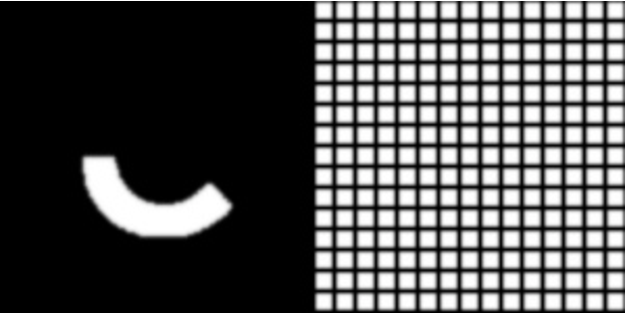
\includegraphics[width=0.32\textwidth]{fig/grid1100} 
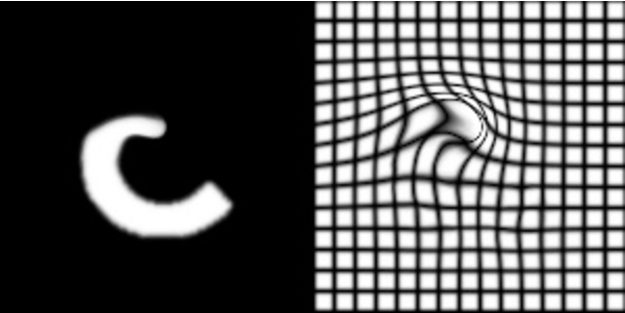
\includegraphics[width=0.32\textwidth]{fig/grid1110} 
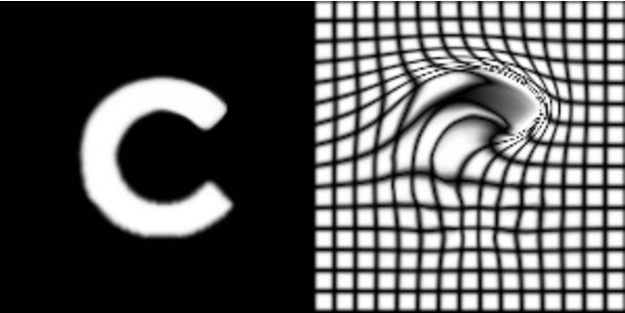
\includegraphics[width=0.32\textwidth]{fig/grid1119} 
\caption{A classical example showing the progress of deforming a half
  C to a full C along a diffeomorphism.  The deforming 
  grid accompanies each deformed image.}
\vspace{-0.1in}
\label{fig:chalf}
\end{figure}


One way to understand these approaches is to study the different forms of parameterization used for the diffeomorphism model. In this paper, we focus on four popular diffeomorphic models: LDDMM from Beg et al \cite{Beg2005Computing},
DARTEL from Ashburner \cite{Ashburner2007}, diffeomorphic demons \cite{Vercauteren2009} and LogDemons \cite{Vercauteren2008Symmetric} from Vercauteren et al. 

Our discussion proceeds in two steps. We first unify the general image registration in the same framework, using the small deformation as examples. We discuss various regularization approaches applied in these
methods and show how they can be unified
using the Sobolev gradient. We explain how the
gradient of the image similarity term is mapped to the transformation space through the regularization term.

After exploiting the shared framework, we focus on discovering the different variants by
contrasting the parameterization of the diffeomorphic transformation
models. We compare the relationship between these algorithms and
discuss how they can be converted to each other by simplifying
assumptions or changing optimization schemes etc. We show that these 
large deformation algorithms may be viewed as
extensions of the common small deformation image registration methods. 

For a clear comparison, the variant notations used by different authors are unified in this paper. We especially fill in the mathematical details, assuming a
common engineering background for readers, to aid in a complete understanding of
the derivation of the most important equations. Many techniques commonly used in diffeomorphism can find roots in the derivation of the small deformation models and the regularization terms. 


There are other important problems in diffeomorphic image registration and we could not cover them in this paper. A few of them include the image  similarity terms, the B-spline transform model, the second-order optimization schemes, the symmetric scheme and inverse consistency problem, the numerical methods with Eulerian and Lagrangian coordinates, and other interesting constraints based on the velocity parameterization. 



% \section{mathematical notation}

\newcommand{\vect}[1]{\mathbf{#1}}
\newcommand{\field}[1]{\mathbf{#1}}
\newcommand{\image}[1]{#1}
\newcommand{\I}{\image{I}}
\newcommand{\J}{\image{J}}
\renewcommand{\u}{\vect{u}}
\renewcommand{\v}{\vect{v}}
\renewcommand{\c}{\vect{c}}
\newcommand{\h}{\vect{h}}
\newcommand{\w}{\vect{w}}
\newcommand{\myphi}{\phi}
\newcommand{\mypsi}{\psi}
\newcommand{\D}{D}
\renewcommand{\d}{\nabla}
\newcommand{\dd}{\text{d}}
\newcommand{\p}{\partial}
\renewcommand{\L}{\Delta} % laplacian
\newcommand{\R}{\mathbb{R}}
\newcommand{\myS}{S}
\newcommand{\myR}{R}
\newcommand{\myE}{E}
\newcommand{\ld}{\langle}
\newcommand{\rd}{\rangle}
\newcommand{\LL}{\mathcal{L}} % operator L
\newcommand{\tQ}{\mathcal{Q}}
\newcommand{\Id}{\text{Id}}
\newcommand{\tG}{{G}} % operator L
\newcommand{\Diff}{\text{Diff}}
\newcommand{\VV}{\mathcal{V}}
\newcommand{\opL}{\mathcal{L}}

\section{From Small Deformation to Large Deformation in Image Registration}

The goal of image registration is to find a viable transform from one image to the other. Such a transform defines pixel-wise correspondences between two images. 
To simplify notation, we assume that any image $\I$ discussed here is a scalar function defined on the same spatial domain: $\I$ : $\Omega \subseteq \R^d \to \R$. 
For example, a 3D image has $d=3$. A transform $\myphi$ is a mapping between two spatial domains: $\Omega \rightarrow \Omega$. 
If one transform $\myphi$ is applied to an image $I$, a new warped
image is generated as the composition of two functions $\I \circ
\myphi$, which is also a function $\Omega \to \R$. 

Given an template image $\I_0$ (i.e. \textit{the fixed image}) and an
individual image to be warped $\I_1$ (i.e. \textit{the moving image}),
the image registration problem optimizes a transform $\myphi$ such
that the warped moving image $\I_1 \circ \myphi$ is close to the fixed image $\I_0$ and $\myphi$ is smooth. 
This is formulated as minimization of an energy function
$\myE(\myphi)$, which usually comprises two parts:
\begin{align}
\label{eq:energy}
\myE(\myphi) = \lambda_S \myS(\I_0,\I_1,\myphi) + \lambda_R \myR(\myphi),
\end{align}
in which $\lambda_S$ and $\lambda_R$ are two scalar weights. The first term in the right is an image similarity function $\myS(\I_0, \I_1, \myphi)$, evaluating the similarity between two images using the transform $\myphi$. 
How to choose an appropriate similarity function is a fundamental problem in image registration, which, however, is not a topic in this paper. 
Here we adopt the sum of square difference (SSD) of two images as the
similarity function throughout this paper, for both its simplicity and
familiarity. One can write SSD as:
\begin{align}
\myS(\I_0, \I_1, \myphi) = \| \I_1 \circ \myphi - \I_0 \|^2.
\label{eq:SSD}
\end{align}

The second part is a transform regularization function $\myR(\myphi)$,
which is usually solely defined on the transform. This term is a prior
on the transform smoothness. For some specific parameterized transformation model, for example, the affine transformation or the B-spline transformation, the smoothness is implicitly encoded through corresponding parameterization forms. 
However, for general non-rigid registration when no other information is available, the transform $\myphi$ is defined using a deformation vector field $\u$: $\Omega \to \R$,
\begin{align}
\myphi(x) = x + \u(x), \; x \in \Omega.
\end{align}
Such a parameterization is simply adding an identity transform with a vector field. 
Regularization functions are normally defined on $\u$ instead of directly on $\myphi$.
% Later we may simply denote a transform $\myphi$ using $\u$ for simplicity. 
$\u(x)$ is a zero vector field when $\myphi(x)=x$. 
This form is strongly connected to Hooke's law about the equilibrium position of elastic material.

In the rest of this section we particularly elaborate on the mathematical details for the easy understanding of the derivation details, which is important on the discussion of large deformation models.



\subsection{A First Example: Horn-Schunck Optical Flow}
\label{sec:opticalflow}
There are many choices of regularization terms. One simple model is to
constrain first order variation of the displacement field $\u$. This
is denoted as the membrane energy model \cite{Ashburner2007} and
provides one form of Tikhonov regularization \cite{Horn1981}:
\begin{align}
\label{eq:membrane}
\myR(\u) = \frac{1}{2} \int_\Omega \sum_{i=1}^d\sum_{j=1}^d (\frac{\p \u_i(x)}{\p x_j})^2 \dd x
= \frac{1}{2} \int_\Omega \sum_{i=1}^d \| \d \u_i(x) \|^2 \dd x = \frac{1}{2} \int_\Omega \| \d\u(x)\|^2 \dd x.
\end{align}
Solving the Euler-Lagrangian equation of this functional gives the negative Laplacian function as its derivative:
\begin{align}
\label{eq:membraneEL}
\frac{\p R(\u)}{\p \u_i} = -  \sum_{j=1}^d \frac{\p^2 \u_i(x)}{\p x_j^2} 
= -  \L \u_i(x) 
, \; i=1 \cdots d \;.
\end{align}
When $\u$ is close to zero, the SSD function of Eq.\ref{eq:SSD} can be approximated using the first order Taylor expansion:
\begin{align}
\I_1 \circ (x + \u ) - \I_0 \approx (\I_1 - \I_0 ) + \ld u, \d I_1(x) \rd
\label{eq:approxopticalflow}
\end{align}

Combining it with the Tikhonov regularization leads to the overall energy function of Horn-Schunck optical flow method: 
\begin{align}
\myE(\u) = \lambda_S \int_\Omega ((\I_1 - \I_0 ) + \ld \u, \d I_1 \rd)^2 \dd x
+ \lambda_R \int_\Omega \sum_{i=1}^d \| \d \u_i(x) \|^2 \dd x
\end{align}

The Euler-Lagrangian equations of $\myE(\u)$ at each pixel $x$ gives the linear system of the optimal point:
\begin{align}
\lambda_S (\I_1 - \I_0  + \ld \u, \d I_1(x) \rd) \frac{\p I_1(x)}{\p x_i}
- \lambda_R \L \u_i(x) = 0
, \; i=1 \cdots d
\label{eq:opticalflow}
\end{align}
An iterative optimization scheme was given in \cite{Horn1981}, which is essentially the Jacobi method of solving the large sparse linear system. Such a method only works for small $\u$. However we are going to reformulate it and explore some important ideas adopted in large deformation methods. 

Notice that the first term in the left is the derivative of the image similarity function and the second term is the derivative of the regularization function, we actually have a general form of the functional derivative as:
\begin{align}
\d_\u \myE(\u) = \d_\u \myS(\u) + \d_\u \myR(\u).
\end{align}


Various optimization schemes can be derived from this representation. For example, the steepest gradient descent is an iterative scheme as $\u \leftarrow \u - \epsilon \d \myE(u)$. By introducing the second order approximation of $\myE(\u)$, one can apply Gauss-Newton method, Levenberg-Marquardt algorithm, or the Newton method when the second order derivative of $\myE$ is feasible. In this paper we mostly focused on the derivation of the first order gradient.

The optimal point can also be computed by iteratively solving the linear system $\d_u \myE = 0$. 
Specifically if we denote $\tQ$ as an operator on $\u$: $\tQ(\u) = \d_\u \myR(\u)$, we have $\d_\u \myS(\u) + \tQ(\u) = 0$. $\u$ is solved as: 
\begin{align}
\u = \tQ^{-1}(-\d_\u \myS(\u))
\label{eq:projection}
\end{align}
As the regularization $\myR$ is solely defined on $\u$, $\tQ^{-1}$ is
independent of choice of $\myS$. This formulation now can be viewed as
projecting of $-\d_\u \myS(\u)$ to a new vector space. Each iteration
consists of two steps. The first gives the initial estimate of the displacement from the image observation. The second regularizes the estimate by projecting it to a smooth vector space. Such a two step approach is practically adopted in the optimization of many image registration algorithms and we will elaborate on this later.

For Horn-Schunck optical flow, $\tQ^{-1}$ is indeed the inverse
operator of Laplacian and thus filters out high-frequency components
of the deformation field $\u$ in the Fourier domain. Later we will
also analyze other transformation models through the perspective of
projecting the similarity function gradient to the vector space.	





% \begin{align}
% & \image{I_1} - \image{I_0 \circ \varphi} \\
% & \varphi(x) = x + \vect{u}(x) \\
% & \varphi(x) = x + \exp(\vect{v}(x)) \\
% & \I_0 - \I_1 \circ \myphi \\
% & \myphi(x) = x + \u(x) \\
% & \myphi(x) = x + \exp(\v(x)) \\
% % & \D  \myphi = \frac{\partial \myphi}{\partial x} \\
% % & \D \myphi \circ \myphi(x,t) \\
% % & \D \myphi | _{ \myphi(x,t) } \\
% % & \D (g \circ h)  = \D g |_{h(x)} \D h \\ 
% % & \D (g \circ h)  = \D g  \circ {h(x)} \D h \\ 
% & \D_{x} (g \circ h)  = \D_{h(x)} g  \, \D h \\ 
% & |\D \myphi |   \\
% \end{align}


\subsection{Demons algorithm}
\label{sec:demons}

Before introducing image registration of large deformation, we briefly
go over another important small deformation registration method:
Thirion's demons algorithm \cite{Thirion98}.  The demons algorithm is
one efficient method applied in medical image
registration and has many variants. It also serves as a baseline algorithm of other large deformation models. 

In Thirion's original paper \cite{Thirion98}, the demons algorithm considered the image registration as a diffusion process. The pixels of images were pushed by demons with local forces inspired by optical flow equations. However, the diffusion scheme was described more or less like a heuristic procedure without a clear theoretical explanation. Cachier et al \cite{Cachier2003} justified the algorithm as an alternating minimization of an energy function. The idea is to introduce an auxiliary variable of $\c$ as the raw correspondences between pixels, which can be viewed as the observation of the underlying transform $\myphi$:
\begin{align}
\myE(\myphi,\c)= \frac{1}{\sigma_i^2}\| \I_1 \circ \c - \I_0 \|^2
+\frac{1}{\sigma_x^2} \|\c - \myphi\|^2
+\frac{1}{\sigma_T^2} \int_\Omega \| \d\u(x)\|^2 \dd x,
\end{align}
where $\sigma_i$ accounts for the noise on the image intensity, $\sigma_x$ accounts for a spatial uncertainty on the correspondences and $\sigma_T$ controls the amount of regularization. Now the demons algorithm is explained as an alternating optimization over $\c$ and $\myphi$. The first step solves for $\c$ by optimizing $\myS(\c) = \frac{1}{\sigma_i^2}\| \I_1 \circ \c - \I_0 \|^2 +\frac{1}{\sigma_x^2} \|\c - \myphi\|^2 $ given current $\myphi$. 
This is similar to the optical flow equation with the constraint that $\c$ should be close to $\myphi$. 
The second step solves for $\myphi$ by optimizing $\myR(\myphi) = \frac{1}{\sigma_x^2} \|\c - \myphi\|^2+\frac{1}{\sigma_T^2} \int_\Omega \| \d\u(x)\|^2 \dd x$ with given $\c$. 
This is actually the projection step we discussed in the last
section. $c$ and $\myphi$ are typically initialized as the identity transform.

Since $\c$ and $\myphi$ have to be close, let $\c = \myphi + \w$ . The minimization of $\myS(\c)$ here used the same first order expansion of $I_1 \circ \c $ as in the optical flow algorithm:
\begin{align}
\myS(\c) = \myS(\myphi+\w) \approx
\frac{1}{\sigma_i^2} ( \I_1 \circ \myphi - \I_0 + \ld \w, \d_{\myphi} \I_1 ) \rd )^2 
+ \frac{1}{\sigma_x^2} \| \w \|^2,
\end{align}
where $\d_{\myphi}\I_1$ means $(\d\I_1)(\myphi)$. The optimal $\w$ is now given by 
\begin{align}
\left( \d_{\myphi}\I_1 \d_{\myphi}^T \I_1 
      + \frac{\sigma_i^2}{\sigma_x^2}  
\right) \w 
+ (\I_1 \circ \myphi - \I_0 )\d_{\myphi}\I_1 = 0
\end{align}
Using the Sherman-Morrison formula, the solution yields one choice of demon displacement $w$ as:
\begin{align}
\w = -\frac{\I_1 \circ \myphi - \I_0 }
           {\|\d_{\myphi}\I_1\|^2 + {\sigma_i^2}/{\sigma_x^2}}
           \d_{\myphi}\I_1
\label{eq:adddemonforce}           
\end{align}

Optimizing $\myphi$ (or $\u = \myphi - x$) given the auxiliary variable $\c$ is a quadratic form: 
\begin{align}
\myR(\myphi) = \frac{1}{\sigma_x^2} \|\c - \myphi\|^2+\frac{1}{\sigma_T^2} \int_\Omega \| \d\u(x)\|^2 \dd x,
\end{align}
which has a closed form solution.  Using the Euler-Lagrangian equation yields the optimal $\u$ given $\c$ as:
\begin{align}
\u = \left( \Id - \frac{\sigma_x^2}{\sigma_T^2} \L \right)^{-1} \left( \c - x \right),
\end{align}
where $\Id$ is the identity operator. Comparing this with
Eq.\ref{eq:projection}, now it is clear that this regularization step
is also projecting the auxiliary variable $\c-x$ using a smoothing
operator  $\tQ^{-1} = \left( \Id - {\sigma_x^2}/{\sigma_T^2} \L \right)^{-1}$. 
Thirion's demons algorithm applies Gaussian smoothing for efficient
computation: $\tQ^{-1} \u = \tG \ast \u$, where $\tG$ is a Gaussian
kernel and $\ast$ represents image convolution. For now let us simply
assume that $\left( \Id - {\sigma_x^2}/{\sigma_T^2} \L \right)^{-1} =
\tG$.  We will come back to the exact regularization terms corresponding to Gaussian smoothing later.

Now we summarize the demons algorithm as:
\begin{algorithm}
\caption{Additive Demons Algorithm}
\label{alg:additivedemons}
\begin{enumerate}
\item{Given current transformation $\myphi$, compute the correspondence update field $\w$ using Eq.\ref{eq:adddemonforce}. 
}
\item{Additive update: $\c \leftarrow \myphi + \w$.
}
\item{Regularization: $\myphi \leftarrow \Id + \tG \ast (\c - \Id)$. Go back to 1.
}
\end{enumerate}
\end{algorithm}

\subsection{Compositive Demons and Inverse Transform}
\label{sec:compositivedemons}

The additive update performs a gradient descent on $\w$ in the vector
space $\R^d$. Another way to combine to $\myphi$ and $\w$ is through composition:
\begin{align}
\c = \myphi \circ \left( \Id + \w \right)
\label{eq:demoncomp}
\end{align}
Its first order approximation at $\w \to 0$ is similar to the additive one: $\c = \myphi + \d\myphi\cdot\w$. The corresponding similarity term is:
\begin{align}
\myS(\c) = \myS(\myphi \circ (\Id + \w) ) \approx
\frac{1}{\sigma_i^2} ( \I_1 \circ \myphi - \I_0 + \ld \w, \d (\I_1 \circ \myphi ) \rd )^2 
+ \frac{1}{\sigma_x^2} \| \w \|^2,
\label{eq:compdemonssim}
\end{align}
and the corresponding demons force $\w$ becomes:
\begin{align}
\w = -\frac{\I_1 \circ \myphi - \I_0 }
           {\|\d (\I_1 \circ \myphi )\|^2 + {\sigma_i^2}/{\sigma_x^2}}
           \d (\I_1 \circ \myphi )
\label{eq:compdemonforce}           
\end{align}

We list the compositive demons algorithm in Alg. \ref{alg:compdemons}. 
If we set $\sigma_i$ as a pixel-wise function: $\sigma_i(x) = \I_1 \circ \myphi - \I_0 $, Eq. \ref{eq:compdemonforce} is close to the form of the original demons force in \cite{Thirion98}. There are other variants of demons forces by choosing different forms of $\myS$ and various second-order optimization schemes. 

\begin{algorithm}
\caption{Compositive Demons Algorithm}
\label{alg:compdemons}
\begin{enumerate}
\item{Given current transformation $\myphi$, compute the correspondence update field $\w$ using Eq.\ref{eq:compdemonforce}. 
}
\item{Additive update: $\c \leftarrow \myphi \circ \left( \Id + \w \right)$.
}
\item{Regularization: $\myphi \leftarrow \Id + \tG \ast (\c - \Id)$. Go back to 1.
}
\end{enumerate}
\end{algorithm}

The compositive demons requires to compute the transform composition $\myphi \circ \left( \Id + \w \right)$ instead of simply adding $\myphi + \w$. It also computes the gradient of the warped image $\I_1$ as $\d (\I_1 \circ \myphi)$ (Eq. \ref{eq:compdemonforce}). In contrast, the additive update needs to warp the gradient image: $\d_{\myphi}\I_1$ (Eq. \ref{eq:adddemonforce}), which may have higher numerical error since the gradient image is usually a sparse image.

A more important difference between the compositive and the additive update schemes is related to the invertibility of the transforms. 
When $\w$ is small, it is approximated that $\Id+\w$ is invertible
with $(\Id+\w)^{-1}=\Id-\w$. But this is generally false for large deformation $\w$. An example was illustrated in \cite{Ashburner2007} (see Fig.\ref{fig:smallinverse}). 
In the additive update scheme $\c \leftarrow \myphi + \w$, $\c$ usually quickly becomes non-invertible after several iterations. The adding operation in the vector space does not preserve invertibility. 

\begin{figure}
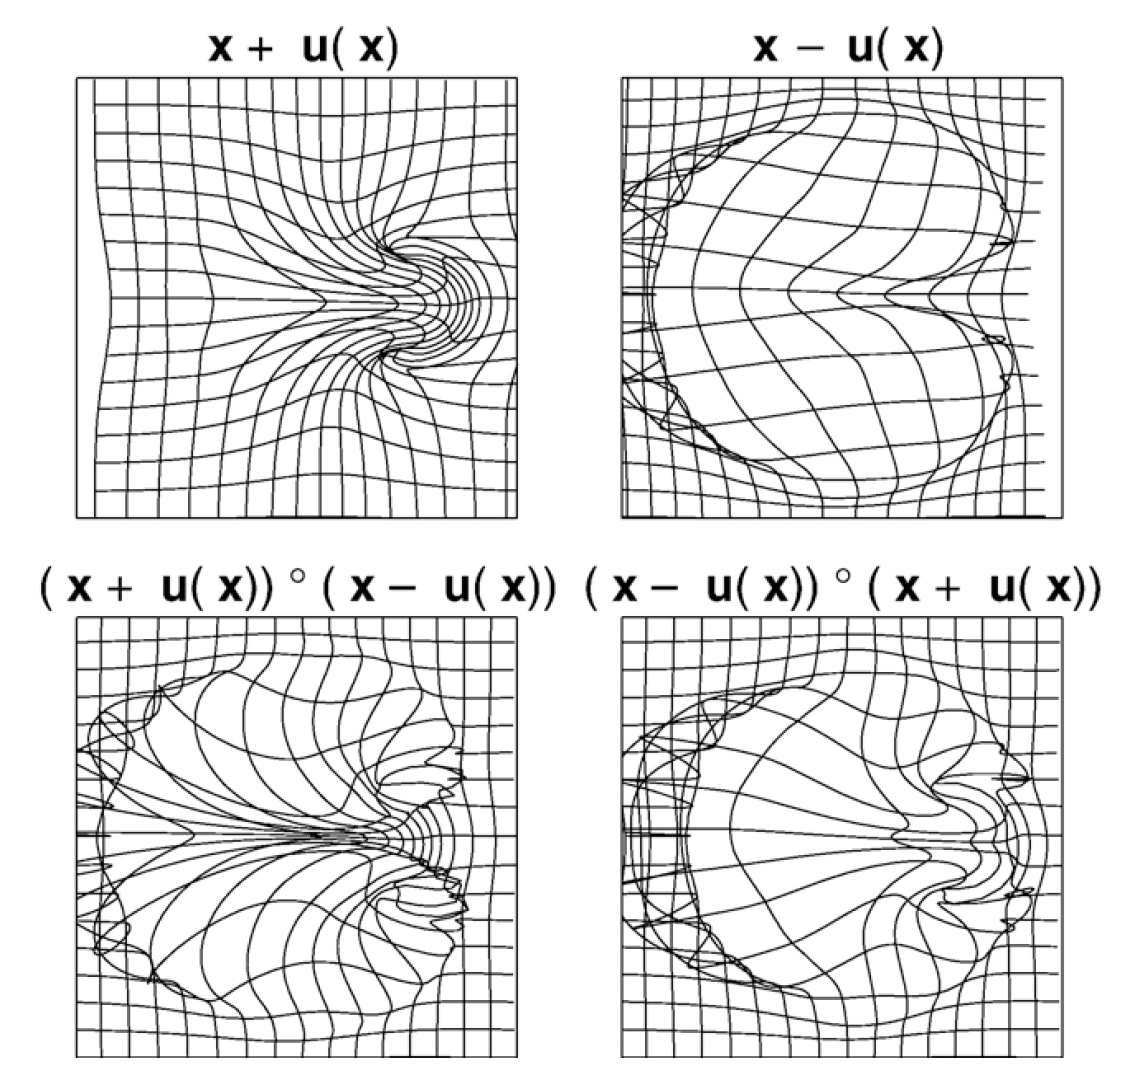
\includegraphics[width=0.8\textwidth]{fig/smallinverse}
\caption{\label{fig:smallinverse}
Fig.1 from \cite{Ashburner2007}. Inversion and composition in a small deformation setting. The compositions are not identity transform.
}
\end{figure}


On the other side, the composition of two invertible transforms is still invertible. 
This implies that the compositive scheme is able to yield an invertible transform when $\w$ is small in each iteration, which was validated in \cite{Vercauteren2009}. 
This means that a large and invertible transform is able to be generated from the composition of many small deformation fields. In the following sections we are going to formalize this intuition and
reveal this as the background for many large deformation transformation models.

\subsection{Diffeomorphism Group}
\label{sec:diffgroup}

The small deformation algorithms we discussed before parameterize the
transform as $\myphi(x) = x + \u(x)$. Unless $\u(x)$ is close to
zero, such a form is not necessarily invertible and in general cannot
preserve topology. In many applications, the nonrigid transform
between two images are very large, where 'large' is defined in a
historical context, that is, relative to transformations typically
captured by elastic or demons type algorithms. Traditionally, these
small deformation algorithms could not both explicitly enforce a
one-to-one mapping and provide a high-quality registration
solution. It is therefore necessary to exploit the large deformation
framework which can preserve topology while capturing a wide range of transformations.

Large deformation is conveniently represented as a diffeomorphism in
mathematics. A diffeomorphism $\myphi$ is a globally one-to-one
continuous and smooth mapping with a continuous and smooth inverse. In other words, $\myphi^{-1}$ exists and both $\myphi$ and $\myphi^{-1}$ are invertible. The diffeomorphism forms a group $\Diff$ under the composition operation, i.e. $\myphi_1 \circ \myphi_2 \in \Diff$ when $\myphi_1, \myphi_2 \in \Diff$:
\begin{align}
\Diff = \{ \myphi: \Omega \to \Omega | \myphi \text{ and } \myphi^{-1} \text{ are differentiable }\}.
\end{align}

Suppose there are a series of small deformations $(\mypsi_k \in \Diff)_{0 \leq k \leq n}$, we recursively define $\myphi_0 = \Id$ and $\myphi_{k+1} = \myphi_{k} \circ \mypsi_{k}$.  $(\myphi_{k})$ forms a polygonal line in $\Diff$. Note that the solution of compositive demons falls into this representation. In a continuous setting this polygonal line become a curve: $\myphi(x, t), \, 0 \leq t \leq 1$. Here $t$ is a time variable and $\myphi(x, t)$ is the position of one particle whose position was $x$ when $t=0$.

When $\myphi(x, t)$ is differentiable in $t$, we have the important o.d.e that generates a diffeomorphism:
\begin{align}
\frac{\dd}{\dd t} \myphi(x, t) = \v(\myphi(x, t), t), 
\label{eq:ode}
\end{align}
where $\v$ satisfies continuity conditions in order to guarantee the
existence of the solution. But it is important to point out that
$\v(x,t)$ does not need to be invertible w.r.t $x$.

By introducing the time variable $t$, we can define a curve of transformations between two images $\I_0$ and $\I_1$. Define $\myphi_t$ as the transform time $t$ and similarly for $\v_t$:
\begin{align}
& \myphi_t(x) = \myphi(x, t) \\
& \v_t(x) = \v(x, t) \\
\end{align}

At time $t=0$, $\myphi_0 = \Id$; at time $t=1$, we get the final
transform $\myphi = \myphi_1$. Since $\myphi_t$ has an inverse transform, we can also define the transform between two time points $\myphi_{s,t}$ as:
\begin{align}
\myphi_{s,t} = \myphi_t \circ (\myphi_s)^{-1}.
\end{align}
We immediately have the following properties:
\begin{align}
& \myphi_{t, s} = \myphi_{s, t}^{-1} \\
& \myphi_{t, s} = \myphi_{r, t} \circ \myphi_{s, r} \\
& \myphi_1 = \myphi_{0, 1} \\
& \myphi_1^{-1} = \myphi_{1, 0}
\label{eq:invphi}
\end{align}

The o.d.e Eq. \ref{eq:ode} gives an important way to parameterize
$\myphi$ with the time-variant velocity fields $\v$. Instead of only
modeling the target transform $\myphi_{0,1}$, such a parameterization
encodes the whole temporal path that determines how one image $I_1$ is
deformed into another image $I_0$. Since $\myphi_t$ is a
diffeomorphism, this path is an invertible one-to-one mapping. An
invertible transform $\myphi_1$ can be constructed from a time-variant
velocity vector fields $\v_t$, which does not need to be
invertible. Such a parameterization of $\myphi$ avoids handling the existence of $\myphi^{-1}$ directly, which is a desirable property. In the following sections we discuss in detail how different approaches compute $\v$ in the setting of image registration. We show the relationship between different diffeomorphism approaches and small deformation algorithms by deriving them from each other.

\subsection{Connection Between Small deformation and Diffeomorphism}

We already saw that the compositive demons is close to large deformation image registration. It is helpful to view Eq. \ref{eq:ode} by discretization of $t$. Suppose we discretize $\myphi_t, \, 0\leq t \leq 1$ into a series of $(\myphi_i)_{0 \leq i \leq N}$, at time $t$:
\begin{equation}
\begin{split}
& \frac{\dd}{\dd t} \myphi_t = \v_t(\myphi_t) \; , \\
& \frac{\myphi_{i+1}-\myphi_{t}}{\delta t} \approx \v_t(\myphi_t) \; , \\
& \myphi_{i+1} = \myphi_{i} + \delta t \v_t \circ \myphi_t \; , \\
& \myphi_{i+1} = (\Id + \delta t \v) \circ \myphi_t \; .\\
\end{split}
\label{eq:discretizeode}
\end{equation}
Let $\w = \delta t \v$ and we have:
\begin{align}
\myphi_{i+1} = (\Id + \w) \circ \myphi_i
\end{align}

Comparing with the composition used in Eq. \ref{eq:demoncomp} we see
the difference is whether the small deformation approximation occurs before or after the last transform $\myphi_i$. The advantage of Eq. \ref{eq:demoncomp} is that it is easier to compute the derivative of $\d_w(\myphi \circ (\Id + \w)) $; but physically it is more natural to compose the update $\w$ after the current transform $\w$. We will discuss the derivation from Beg. et al \cite{Beg2005Computing} in the Sec. \ref{sec:lddmm}.

Another important fact about this discretization is that although $\Id + \v$ is not necessarily invertible, $\Id + \delta t \v$ is usually invertible for a small scalar $\delta$ with $(\Id + \delta t \v)^{-1} \approx \Id - \delta t \v$. Thus $\myphi_N$ is also invertible. We will revisit this in Ashburner's method \cite{Ashburner2007} and Vercauteren's methods \cite{Vercauteren2009, Vercauteren2008Symmetric}.
 
Theoretically we only require $\v$ to be continuous to satisfy the
existence of $\myphi$; it is more desirable that it is also smooth
both for numerical issues and to provide an additional smoothness
control on $\myphi$. The smoothness constraint we discussed before about the small deformation $\w$ is now equivalent to the smoothness of the velocity field $\v$. The regularization term $R(\u)$ where $\u = \myphi - \Id$ naturally becomes a function on $\v$: $R(\v)$.



\section{Smooth Vector Fields and Sobolev Gradient}

Before we discuss various forms of parameterization $\v$ of
diffeomorphism $\myphi$, it is necessary to discuss the regularization
on the vector fields $\v$. A general prior about the final solution of
the optimal transform is that it has to be a smooth one. The main aim
of regularization in diffeomorphic image registration is to guarantee
smoothness of $\v$ under noisy imaging conditions and thus implicitly
of the resulting transform $\myphi$.  Velocity field regularity also
improves stability of the numerical integration scheme for both the
forward and the inverse transform. 

The regularization term is an important factor not only in formulating
the registration energy function itself, but  also in choosing the
corresponding optimization schemes. A vector field $\v$ is usually
defined in an Euclidean space $L^2$ of square integrable
functions. However, this vector space does not have any smoothness
constraints. Hilbert space was introduced in the image registration domain by many researchers \cite{Trouve1998, Beg2005Computing, Hernandez2008, Zikic2010}. Hilbert space can be viewed as a space of smooth functions. This section summarizes the theoretical analysis of regularization as minimizing the image similarity directly in Hilbert space. Using the notion of optimization in Hilbert space we show that various diffeomorphism optimization schemes are unified in the same framework in the later sections.


\subsection{Examples of Regularization Terms and Their optimization Operators}
\label{sec:regularizerexample}

The smoothness of a vector field $\v$ is usually defined using its $k$-th order spatial derivatives. Before the discussion of Hilbert space, it is helpful to revisit the formulation of several common regularization terms used in the literature \cite{Horn1981,Beg2005Computing,Ashburner2007,Vercauteren2009} $\myR(\v)$ and their derivatives $\p\myR/\p\v$, which all can be derived using Euler-Lagrangian equations. Note that it requires the $k$-th order derivatives of $\v$ vanish at the boundary of the domain $\Omega$.

\subsubsection*{Membrane Model}
In Sec. \ref{sec:opticalflow} we already went over the membrane model:
\begin{align}
\label{eq:membraneA}
& \myR(\v) = \frac{1}{2} \int_\Omega \sum_{i=1}^d \| \d \v_i(x) \|^2 \dd x \;, \\
\label{eq:membraneAEL}
& \frac{\p \myR(\v)}{\p \v_i} = -  \L \v_i(x)
, \; i=1 \cdots d \;. 
\end{align}

\subsubsection*{Bending Energy Model}
\begin{align}
& \myR(\v) = \frac{1}{2} \int_\Omega \sum_{i,j,k=1}^d  
\left( 
\frac{\p^2 \v_i(x)}{\p x_j \p x_k}
\right)^2 \dd x 
\\
\label{eq:dbending}
& \frac{\p \myR(\v)}{\p \v_i} 
= 
\sum_{j,k=1}^d
\frac{\p^4 \v_i(x)}{\p x_j^2 \p x_k^2}
=
\L^2 \v_i(x)
, \; i=1 \cdots d \;. 
\end{align}

\subsubsection*{Laplacian model}
\begin{align}
& \myR(\v) = \frac{1}{2} \int_\Omega \sum_{i=1}^d (\L \v_i(x))^2 \dd x
= \frac{1}{2} \int_\Omega \sum_{i=1}^d  
\left( 
\sum_{j=1}^d  
\frac{\p^2 \v_i(x)}{\p x_j^2}
\right)^2 \dd x 
\\
\label{eq:dlaplacian}
& \frac{\p \myR(\v)}{\p \v_i} 
= 
\sum_{j,k=1}^d
\frac{\p^4 \v_i(x)}{\p x_j^2 \p x_k^2}
=
\L^2 \v_i(x)
, \; i=1 \cdots d \;. 
\end{align}
Note that the Laplacian model and Bending model \cite{Ashburner2007}
actually share the same derivation (comparing Eq. \ref{eq:dbending} and Eq. \ref{eq:dlaplacian}).

\subsubsection*{Cauchy-Navier Model}
\label{sec:cauchynaviermodel}

This is used in Beg's paper \cite{Beg2005Computing} and it is a
variant of the Laplacian model. With a little abuse of notation, define the operator $\opL$ as $\opL = \gamma \Id - \alpha \L$:
\begin{align}
& \myR(\v) = \frac{1}{2} \int_\Omega \| \opL \v \| ^2 \dd x
= \frac{1}{2} \int_\Omega \sum_{i=1}^d  
\left(
\gamma \v_i(x) - \alpha \sum_{j=1}^d  \frac{\p^2 \v_i(x)}{\p x_i^2}
\right)^2 \dd x
\\
\end{align}
\begin{equation}
\label{eq:dBeg}
\begin{split}
\frac{\p \myR(\v)}{\p \v_i} 
& = 
\gamma^2 \v_i^2 - 2 \gamma \alpha \sum_{j=1}^d{\frac{\p^2 \v_i(x)}{\p x_i^2}} 
+ \alpha^2 \sum_{j,k=1}^d{\frac{\p^4 \v_i(x)}{\p x_j^2 \p x_k^2}} 
\\
& = (\gamma \Id - \alpha \L)^2 \v_i \\
& = L^2 \v_i
, \; i=1 \cdots d \;.
\end{split} 
\end{equation}

\subsubsection*{Tikhonov Regularization and Gaussian Smoothing}
\label{sec:gaussian}
In Sec. \ref{sec:demons} we conveniently explain how the Gaussian
smoother $\tG$ acts as an inverse operator: $\tG = \left( \Id -
  {\sigma_x^2}/{\sigma_T^2} \L \right)^{-1}$ for some $\L$. Strictly speaking, $\tG$ relates to the general Tikhonov Regularization \cite{Nielsen1997,Mansi2010}\footnote{Note: A typo is in \cite{Mansi2010}: the subscript of the equation in Sec 2.2 should be $1 \leq i_1, \cdots, i_k \leq d$, not $i_1 + \cdots + i_k=k$}:
\begin{align}
\myR(\v) = \frac{1}{2} \int_\Omega \sum_{i=1}^d
\v_i^2(x) + 
\sum_{k=1}^{\infty}
\left(
\sum_{1 \leq j_1, \cdots, j_k \leq d}
\frac{1}{\sigma^{2k} k!} \,
\left(
\frac{\p^k \v_i(x)}{\p x_{j_1} \cdots \p x_{j_k}}
\right)^2
\right)
\dd x
\end{align}
As a practice on solving regularization, we provide the full derivation detail in this section. By applying Euler-Lagrangian, we have:
\begin{equation}
\begin{split}
\frac{\p \myR}{\p \v_i} & = \v_i 
+ \sum_{k=1}^{\infty} 
\sum_{1 \leq j_1, \cdots, j_k \leq d}
\frac{(-1)^k}{\sigma^{2k}k!}
\frac{\p^{2k}}{\p x^2_{j_1} \cdots \p x^2_{j_k}} \v_i \\
& =
\v_i 
+ \sum_{k=1}^{\infty} 
\frac{(-1)^k}{\sigma^{2k}k!}
\left(
\sum_{j=1}^{d}
\frac{\p^{2}}{\p x^2_{j}}  
\right)^k \v_i
\\
& = 
\left(
\Id + \sum_{k=1}^{\infty} 
\frac{(-1)^k}{\sigma^{2k}k!}
\L^k
\right) \v_i \;.
\end{split}
\end{equation}
When $k$ only goes to 1, not $\infty$, $\p \myR / \p \v_i$ becomes $(\Id - 1/\sigma^2 \L)$, which was used in Sec. \ref{sec:demons}. Using the notation of operator $\tQ$ in Eq. \ref{eq:projection}, we can now compute its inverse operator $\tQ^{-1}$ from the Fourier transform of the vector field $\v_i(x)$. Let $\mathcal{F}$ denote the Fourier transform, $\omega$ be the frequency variable, and $\mathcal{F}(\v_i(x)) = \hat{\v}_i(\omega)$. We have
\begin{equation}
\begin{split}
\mathcal{F}\left(
\L^k \v_i(x)
\right)
 & = (-1)^k \omega^{2k} \hat{\v}_i(\omega) 
\\
\mathcal{F}\left( \tQ \v_i(x) \right) 
& = \mathcal{F}\left(
\left(
\Id + \sum_{k=1}^{\infty} 
\frac{(-1)^k}{\sigma^{2k}k!}
\L^k
\right)
\v_i(x)
\right)
\\
& = 
\sum_{k=0}^{\infty} 
\frac{\omega^{2k}}{\sigma^{2k} k!} \hat{\v}_i(\omega)\\
& =
\exp \left(
\frac{\omega^2}{\sigma^2}
\right) \hat{\v}_i(\omega)
\end{split}
\end{equation}
To get the Fourier Transform of operator $\tQ^{-1}$, we simply compute the inverse of the coefficient at each $\xi$:
\begin{equation}
\begin{split}
\mathcal{F}\left( \tQ^{-1} \v_i(x) \right) 
& =
\exp \left(
- \frac{\omega^2}{\sigma^2}
\right) \hat{\v}_i(\omega)
\end{split}
\end{equation}
Now it is clear that the inverse Fourier transform leads to the operator as Gaussian convolution smoother $G$.

\subsection{Sobolev Norm and Sobolev Space}

The various examples of regularization terms $\myR(\v)$ showed in the previous Sec. \ref{sec:regularizerexample} all share the same quadratic form of $k$-th order derivatives. 

\begin{align}
\myR(\v) = \sum_{i=0}^K \lambda_i \ld \v^{(i)}, \v^{(i)} \rd \;,
\end{align}
where $\v^{(i)}$ is the $i$-th order derivative of $\v$. For simplicity, we omit the scalar coefficient $\lambda_i$ in this section. Following the discussion in \cite{Zikic2010}, using the differential operator $\opL = (\D^0, \cdots, \D^k)$ and the $L^2$ norm $\| \cdot \|_{L^2} = \ld \cdot, \cdot \rd$, the Sobolev norm $\ld \cdot, \cdot \rd_{H^k}$ is defined as: 
\begin{align}
\ld \v, \v \rd_{H^k} = \sum_{i=0}^k \ld \v^{(i)}, \v^{(i)} \rd_{L^2} = \ld \opL \v, \opL \v \rd_{L^2} \;.
\end{align}

The quadratic form requires that the square of up to the $k$-th order derivative of smooth function $\v$ is integrable. Thus we formalize it as $\v$ belongs to the Sobolev space $H^k$:  $H^k = \{ f : \| f \|_{H^k} < \infty \}$. For simplicity, we omit $k$ in $H^k$. The inner product in Sobolev space is defined as:
\begin{align}
\ld \u, \v \rd_H = \ld \opL\u, \opL\v \rd_{L^2} = \ld \opL^+\opL \u, \v \rd_{L^2} \;,
\end{align}
where $\opL^+$ is called as the adjoint operator of $\opL$.

Now we can simply write the regularization term $\myR(\v)$ as: $\myR(\v) = \| \v \|_{H^k}$. Moreover the derivative of $\myR(\v)$ has the form:
\begin{align}
\d_\v \myR = \opL^+\opL \v = \left ( \sum_{i=0}^k (-1)^i \L^i \right ) \v\;.
\end{align}


\subsection{Registration in Sobolev Space}

Now we reexamine the image registration energy function Eq. \ref{eq:energy}
\begin{align}
\tag{\ref{eq:energy}}
\myE(\v) = \lambda_S \myS(\I_0,\I_1,\v) + \lambda_R \myR(\v),
\end{align}
Using the notion of the smooth function space $H$, the regularization term $\myR(\v)$ can be replaced by the constraint that $\v \in H$:
\begin{align}
\label{eq:sobolevenergy}
\myE(\v) = \myS(\I_0,\I_1,\v) \text{  , with }  \v \in H \; .
\end{align}

Now the energy is the image similarity term only. Accordingly the optimization needs to be computed in Sobolev space to keep $\v$ remaining in $H$ at each iteration step . Sobolev gradient $(\d_\v E)_H$ is used to replace the previous $L^2$ gradient $(\d_\v E)_{L^2}$. We derive their relationship using the first order Taylor expansion with Sobolev inner product:
\begin{equation}
\begin{split}
\myE(\v + \h) 
& \approx \myE(\v) + \ld (\d_\v\myE)_{L^2} , \h \rd_{L^2} 
\\
& = \myE(\v) + \ld (\d_\v\myE)_{H} , \h \rd_H
\\
& = \myE(\v) + \ld \opL^+\opL (\d_\v\myE)_{H}  , \h \rd_{L^2}
\end{split}
\end{equation}

Thus we can express the Sobolev gradient in terms of the $L^2$ gradient as:
\begin{align}
\label{eq:sobolevgradient}
(\d_\v\myE)_{H} = (\opL^+\opL)^{-1} (\d_\v\myE)_{L^2}
\end{align}

The projecting idea we discussed in deriving Horn-Schunck optical flow Sec. \ref{sec:opticalflow} is now also validated using the Sobolev gradient by comparing Eq. \ref{eq:sobolevgradient} with Eq. \ref{eq:projection}. Also from Sec. \ref{sec:gaussian} we know that the Gaussian smoothing is the inverse operator for the gradient of the first-order Tikhonov regularization. This validates the Gaussian smoothing step used in the demons algorithm Alg.\ref{alg:additivedemons} and \ref{alg:compdemons}. Thus we conclude that various registration algorithms we have discussed can be unified as minimizing the image similarity using the Sobolev gradient on the transform parameter $\v$, which is also true for the diffeomorphic approaches from Beg et al \cite{Beg2005Computing}, Vercauteren et al \cite{Vercauteren2007, Vercauteren2008Symmetric}.



\subsubsection{Sobolev Gradient and Preconditioning}
\label{sec:sobolevprecondition}

Another interesting property about the Sobolev gradient was discussed in \cite{Zikic2010}. If the operator $\opL$ is written as $\opL = (\Id, \opL_1)$, we get:
\begin{align}
\opL^+\opL = \Id + \opL_1^+ \opL_1
\end{align}

Eq. \ref{eq:sobolevgradient} now can also be explained using $\left(
  \Id + \opL_1^+ \opL_1 \right)^{-1}$ as a preconditioner for the
$L^2$ gradient of $(\d_\v\myE)_{L^2}$. This connects the Sobolev
gradient with various Gauss methods with preconditioner like the
Gauss-Newton method and the Levenberg-Marquardt algorithm. Thus we can also unify the Levenberg-Marquardt algorithm applied in Ashburner's method \cite{Ashburner2007}.


\section{Diffeomorphism with Time-varying Velocity Fields}
\label{sec:lddmm}

We have formalized the unifying registration framework using the Sobolev gradient. From this section, we study several forms of parameterization $\v$ applied in large deformation algorithms and discuss the connections among them and with small deformation algorithms.

Small deformation transforms normally use a small displacement field $\u$ to model the mapping $\myphi = x + \u$. In contrast, a large deformation transform introduces an extra time variable $t$ to encode the warping path $\myphi(x,t)$ between two images. The first parameterization is using the o.d.e Eq. \ref{eq:ode}:
\begin{align}
\tag{\ref{eq:ode}}
\frac{\dd}{\dd t} \myphi_t(x) = \v_t(\myphi_t(x)), 
\end{align}

Optimizing the diffeomorphism transform $\myphi$ is equivalent to optimizing the time-varying velocity field $\v_t$. An example of $\v_t$ was illustrated in \cite{Beg2005Computing} (see Fig. \ref{fig:vt}).

\begin{figure}
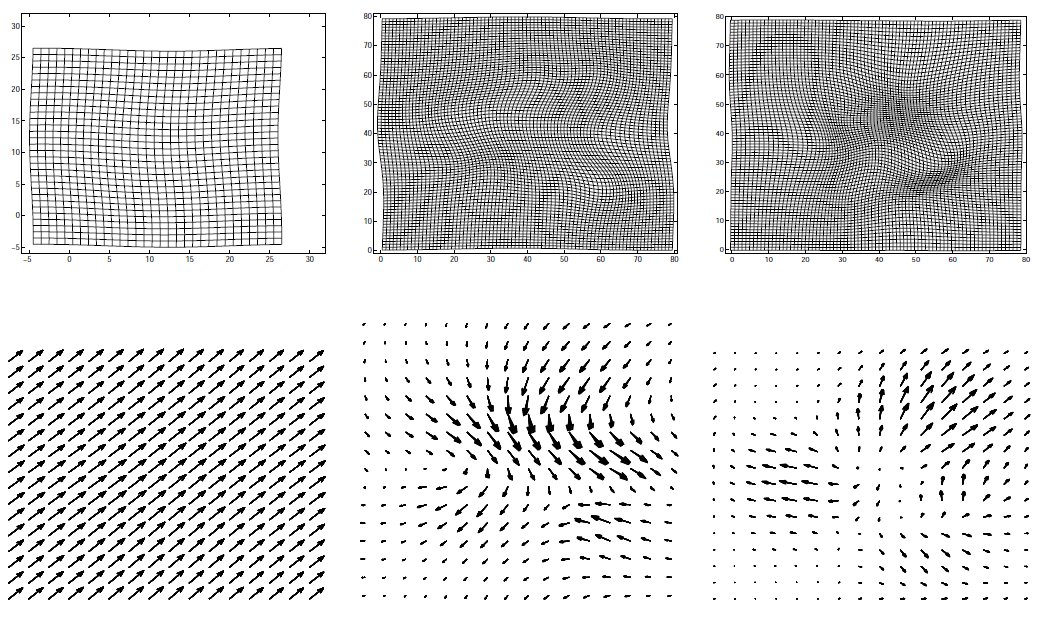
\includegraphics[width=1\textwidth]{fig/vt2}
\caption{\label{fig:vt}
Adapted from of Fig.11 from \cite{Beg2005Computing}. Each column is a pair of $\myphi_1$ (first row) and $\v_t${second row}. Different time points of $\v_t$ are superimposed on the same figure.
}
\end{figure}


\subsection{Beg's LDDMM algorithm}

Beg et al. proposed Large Deformation Diffeomorphic Metric Mapping (LDDMM) algorithm, which used this o.d.e as parameterization to optimize the following energy function:
\begin{align}
\myE(\v) = \frac{1}{2} \| I_0 \circ \myphi_{1,0} - I_1 \|^2 
+ 
\frac{\sigma^2}{2}\int_{0}^{1} \| \opL v_t\|^2 \dd t \;,
\label{eq:lddmm}
\end{align}
where $\myphi_{1,0}$ is defined by Eq. \ref{eq:invphi} in
Sec. \ref{sec:diffgroup}, the operator $\opL$ represents the
Cauchy-Navier regularizer $\myR(\v)$: $\opL = \gamma \Id - \alpha \L$
in Sec. \ref{sec:cauchynaviermodel} with the Hilbert space
$H$. Note that we omit the integral over the spatial domain $\int_x
\cdot\, \dd x$ for simplicity since $\v$ can be reinterpreted as a
vector with an element for each pixel. The image similarity term is
then $\myS(\v) = \frac{1}{2} \| I_0 \circ \myphi_{1,0} - I_1 \|^2 $.

Beg et al gave a rigorous way in computing the derivative of $\d_\v E$ in \cite{Beg2005Computing}. The key in the proof is to introduce the Gateaux variation of $\myphi_{s,t}$ w.r.t $\v$ (Lemma 2.1 from \cite{Beg2005Computing}). A small perturbation of $\v$ at time $r$ (i.e. $h_r$) affects all the transform $\myphi_t$ for $t>r$ cumulatively. 
Since the derivation in \cite{Beg2005Computing} is detailed, we cite this lemma without proof here:
\begin{align}
\p_\h \myphi_{s,t} = \D\myphi_{s,t} 
\int_{s}^{t} 
\left( 
\D \myphi_{s,r}
\right)
^{-1} \h_r \circ \myphi_{s, r} dr
\end{align}

Although it is hard to define the Fr{\'e}chet derivative for $\myphi$, which means that the simple chain rule could not be applied directly to compute $\d_\v \myS$, Beg however showed that $\p_\v \myS$ still has a nice structure related to the Fr\'echet derivative (see the proof of Theorem 2.1 in \cite{Beg2005Computing}):
\begin{align}
\p_\h \myS(\v) = - \int_{0}^{1} 
\ld
|\D\myphi_{t,1}|
(\J_t^0 - \J_t^1)
\D(\J_t^0)
,
\h_t
\rd
\dd t \; ,
\label{eq:lddmmds}
\end{align}
where $\J_t^0 = \I_{0}\circ \myphi_{t,0}$, $\J_t^1 = \I_{1}\circ \myphi_{t,1}$, $D$ is the Jacobian matrix and $\| \cdot \|$ is the determinant value of the matrix.
For the regularization term, the Gateaux variation is easy to compute:
\begin{align}
\p_\h \myR(\v) = \sigma^2 \int_{0}^{1} 
\ld
\opL^+\opL \v_t, \h_t
\rd \dd t
\end{align}
Now the overall Gateaux variation $\p_h \myE(\v)$ can be represented as:
% \begin{align}
$\p_\h \myE(\v) = \int_0^1
\ld
\d_{\v_t} \myE_t , \h_t
\rd \dd t $
% \; ,
% \end{align}
and $\d_{\v_t} \myE_t$ is defined as:
\begin{align}
\d_{\v_t} \myE_t = \opL^+\opL (\sigma^2 \v_t) - |\D\myphi_{t,1}|(\J_t^0 - \J_t^1)\D(\J_t^0)
\label{eq:lddmmgrad}
\end{align}

Beg et al proposed to use the Sobolev gradient instead of this $L^2$ gradient. From Eq. \ref{eq:sobolevgradient}, we get the gradient:
\begin{align}
(\d_{\v_t} \myE_t)_H = \sigma^2 \v_t - (\opL^+\opL)^{-1}(|\D\myphi_{t,1}|(\J_t^0 - \J_t^1)\D(\J_t^0))
\end{align}

\subsection{Numerical Algorithm of LDDMM}
\label{sec:lddmmalg}
In its numerical implementation, the time-varying velocity fields are discretized into $N$ time points $(v_{t_i} )_{0 \leq i \leq N-1}$. For each time point $i$, a standard steepest descent scheme is applied:
\begin{align}
\v_{t_i}  \leftarrow \v_{t_i} - \epsilon (\d_{\v_{t_i}} \myE_{t_i})_H \; .
\end{align}
The inverse of $\opL^+\opL$ in the Sobolev gradient can be computed from the Fourier domain.


One has to compute $\myphi_{t,1}$ and $\myphi_{t,0}$ for $(\d_{\v_{t_i}} \myE_{t_i})_H$ from Eq. \ref{eq:lddmmds}. $\myphi_{t,1}$ can be computed directly by composing $ (1/N)\myphi_{t_{N-1}} \circ \cdots \circ (1/N) \myphi_{t_{i}}$. For $\myphi_{t,0}$, one needs to compute the inverse of $\myphi_{0,t}$. Beg proposed to use a  Semi-Lagrangian scheme in Sec. 3.3 of \cite{Beg2005Computing} for stable numerical computation, which is not covered in this paper. But in general to get the inverse transform is computationally intensive using a series of $v_t$. 

LDDMM method requires that one store $N$ velocity fields. In each iteration, it needs to compute also $N$ gradient fields, $N$ compositions for $\myphi_{t,1}$ and solve $N$ inverse problems. Overall, this is a very expensive algorithm.


\subsection{Comparison with Horn-Schunck Optical Flow}

Revisiting the Horn-Schunck optical flow update Eq. \ref{eq:opticalflow} with the approximation Eq. \ref{eq:approxopticalflow}, one can rewrite it as:
\begin{align}
\d_\u\myE = (\I_0 \circ \myphi - \I_1) \D\I_1 - \lambda \L \u \;.
\end{align}
Comparing with the gradient at time $t$ of LDDMM (Eq. \ref{eq:lddmmgrad}), $\d_{\v_t} \myE_t$ is conveniently explained as the optical flow between $J_t^0$ and $J_t^1$ at time $t$, weighted by the Jacobian determinant $|\D\myphi_{t,1}|$ introduced by change of variable of $ y = \myphi_{t,1}(x)$.\footnote{One small difference is that the image similarity is defined as $\|I_0 \circ \myphi_{1,0} - I_1\|^2$, not $\|I_1 \circ \myphi_{0,1} - I_0\|^2$ (Eq.\ref{eq:SSD}). } 

Thus the LDDMM algorithm can be summarized as computing $v_{t_i}$ in the way of the optical flow for all time $t_i$ and composing all $(v_{t_i})$ to get $\myphi_{t, 1}$ and $\myphi_{t, 0}$.


\subsection{Comparison with Compositive Demons}

Compositive demons described in \ref{sec:compositivedemons} can also be viewed as a greedy optimization of LDDMM. In compositive demons, when the iterative optimization procedure uses iterations, the update $\w_i, 1 \leq i \leq N$ from each iteration can be viewed as the velocity fields. At iteration $i$, the greedy optimization fixes all the velocity fields obtained before $i$ and only optimize $\w_i$. 

The advantage of such a greedy way is that this does not require to store all the velocity fields before $i$, only their composition is needed. The disadvantage of such a greedy method does not put any constraint on the overall quality of $\w_i$. Each $\w_i$ is a local optimal but the transform path following all $w_i$ may be very curvy. In fact, Beg et al also \cite{Beg2005Computing} showed that the regularization used in LDDMM has the same optimal transform as the shortest path to $\Id$.


\section{Diffeomorphism with Stationary Velocity Fields}

The LDDMM method \cite{Beg2005Computing} uses the time varying
velocity fields $\v_t$ to parameterize the diffeomorphism
$\myphi$. Although the derivation is rigorous, the algorithm has a high complexity and also requires stable numerical methods in solving the inverse transform. One way to simplify the problem is to use stationary velocity fields $\v$, which does not change across time, to generate the diffeomorphism \cite{Arsigny2006,Ashburner2007,Vercauteren2007,Vercauteren2008Symmetric,Hernandez2009}. The o.d.e that generates the diffeomorphism is now written as:
\begin{align}
\frac{\dd}{\dd t} \myphi_t(x) = \v(\myphi_t(x)), 
\end{align}

The stationary velocity field $\v$ is referred as the one-parameter generator of a subgroup $\Phi=(\exp(t\v))_{t \in \R}$, where $\v$ belongs to the tangent space of $\Phi$. The final transform is parameterized as the exponential at unit time $\exp(\v)$. The theory about such an infinite-dimensional space with a Lie group structure is still under research \cite{Arsigny2006, Vercauteren2008Symmetric, Sternberg1964, Mahony2002}.  

Using a stationary velocity field $\v$ to replace the time varying velocity fields $\v_t$ greatly simplify the computation. Especially we have
\begin{align}
\myphi_{s,t} = \myphi_{t-s} = \exp((t-s)v)
\end{align}
This shows that using stationary velocity fields, $\myphi_{s,t}$ only depends on the length between two time points and not on the starting point. 

Although not every diffeomorphism can be parameterized by stationary velocity fields \cite{Ashburner2007}, such a model performs well empirically for medical image registration \cite{Hernandez2009, Vercauteren2009}. Parameterization of stationary velocity fields not only simplifies the computation; it also provides the possibility of statistics study using one velocity field, which is desirable in many applications.



\subsection{Computation of Exponential Mapping}

In Sec. \ref{sec:lddmmalg} we discussed that computing $\myphi$
requiring $N$ times composition of vector fields and solve $N$ steps of 
the p.d.e of the inverse transform $\myphi^{-1}$. \footnote{In fact,
  this is the minimal amount of computation required.  Increased
  integration accuracy requires a dense sampling of the o.d.e. in time
  and can require many more integration points than discretization
  points, in particular if an accurate/consistent forward and inverse
  transformation is desired.}  With the stationary field, such complexity can be reduced to $\log N$ times composition for both $\myphi$ and $\myphi^{-1}$. 

Arsigny et al \cite{Arsigny2006} introduced an efficient method to compute the exponential mapping $\myphi = \exp(\u)$ by exploiting the following property:
\begin{align}
\exp(\v) = \exp(N^{-1} \v )^N \;\text{for integer } N.
\end{align}
Using the first order approximation $\exp(N^{-1} \v) \approx \Id + N^{-1}\v$ for sufficiently large $N$, the following "scaling and squaring" algorithm (Alg.\ref{alg:exp}) computes recursively $K$ times for $N = 2^K$:
\begin{algorithm}
\caption{Scaling-and-squaring for Exponential Mapping}
\label{alg:exp}
\begin{enumerate}
\item{Scaling: choose $K$ s.t $2^{-K}\v$ is close to 0, e.g, $\max_x x\|2^{-K}\v(x)\| leq 0.5 $. 
}
\item{First-order approximation: $\myphi^{0} =  \Id + N^{-1}\v \approx \exp(2^{-N} \v) $.
}
\item{Squaring: recursive $K$ steps $\myphi^{k+1} \leftarrow \myphi^{k} \circ \myphi^{k}$. 
}
\end{enumerate}
\end{algorithm}

Another important advantage is that one can also compute $\myphi^{-1}$, the inverse of $\myphi$, using the same scaling-and-squaring method with $\exp(-N^{-1} \v) \approx \Id - N^{-1}\v$. 


\subsection{Ashburner's DARTEL algorithm}

Ashburner proposed to use stationary velocity field for diffeomorphic image registration. The algorithm was named DARTEL: Diffeomorphic Anatomical Registration using Exponentiated Lie algebra. DARTEL can be viewed as a stationary version of LDDMM in many ways. DARTEL uses the image registration energy  function as:
% \footnote{Actually not exactly the same form. Ashburner defined the image similarity term as $\| I_1 \circ \myphi_{0,1} - I_0 \|^2$, here we reformulate it for consistency with LDDMM.}
%  Eq. \ref{eq:lddmm} as:

\begin{align}
\myE(\v) = \frac{1}{2} \| I_0 - I_1 \circ \myphi_{1} \|^2 
+ 
\frac{\sigma^2}{2} \| \opL \v\|^2  \;,
\label{eq:dartel}
\end{align}

Compared with Eq. \ref{eq:lddmmgrad}, the $L^2$ first order derivative of $\myS$ becomes:
\begin{align}
\d_\v \myS(\v) = \int_{0}^{1} 
|\D\myphi_{-t}|
(\I_0 \circ \myphi_{-t} - \I_1 \circ \myphi_{1-t})
\D(\I_1 \circ \myphi_{1-t})
\, \dd t \; ,
\label{eq:dartelds}
\end{align}

Previously we discussed that it is expensive to compute this gradient in LDDMM. But luckily, Ashburner \cite{Ashburner2007} also derived a recursive scheme for $\d_\v \myS(\v)$ using $\log N$ times operation. Using together the scaling-and-squaring algorithm to compute $\myphi$, each gradient update altogether only needs $\log N$ steps of operation. 
% For the sake of completeness, we include it here.
% By discretizing time $0$ to $1$ into $N=2^K$ time points, Eq. \ref{eq:dartelds} becomes:
% \begin{equation}
% \begin{split}
% \d_\v \myS(\v) & = 
% \frac{1}{N} \sum_{n=0}^{N-1} |\D\myphi_{t_n,1}| 
% (\I_1 \circ \myphi_{t_n} - \I_0\circ\myphi_{t_n}^0) \D(\J_{t_n}^0) 
% \\
% & =
% \frac{1}{N} \sum_{n=0}^{N-1} |\D\myphi_{t_n,1}| (\J_{t_n}^1 - \J_{t_n}^0) \D(\J_{t_n}^0) 
% \\
% \end{split}
% \end{equation}

Ashburner used the Levenberg-Marquardt algorithm in $L^2$ space as the optimization scheme, for which the second order derivatives of the energy also was computed. From the discussion in Sec. \ref{sec:sobolevprecondition}, one could also choose to use the gradient descent in the Sobolev space acting as the preconditioner, which was used in Beg et al's LDDMM algorithm \cite{Beg2005Computing}. 

% \subsection{DARTEL regularization and Gauss-Newton Method to Sobolev gradient}
\subsubsection{Comparison with LDDMM}

DARTEL and LDDMM both models the transform from the o.d.e generator. Both algorithms compute the integration over time using $N$ discretized time points. Both have a rigorous derivation of the energy gradient. 
However, the DARTEL algorithm used the stationary velocity field $\v$
as the parameterization of the transform $\myphi$. DARTEL is a simplified way to approximate LDDMM by approximating the velocity fields at all time points with their average.

The DARTEL update of the velocity field can be viewed as the average
of the optical flow at every time point. Instead of having to store
the velocity field at every time point, DARTEL only stores one
velocity field. LDDMM needs to compose (minimum) $N$ different velocity fields to get the transform and compute the gradient at each time point. DARTEL only needs $\log N$ times composition to compute both transform and the gradient. 

Another difference between DARTEL and LDDMM is whether the
optimization occurs in$L^2$ space or the Sobolev space. DARTEL
computes sparse matrix inverse used in each Levenberg-Marquardt
iteration. Although Ashburner proposed to use the multi-grid method with
Gauss-Seidel iteration, such a computation still has high complexity compared to the convolution approach in the Fourier domain used in LDDMM. The higher frequency in the operator $\opL^+\opL$ used in $L^2$ gradient also leads to numerical instability.



\subsection{Vercauteren's Diffeomorphic Demons Algorithm}

Vercauteren extended the compositive demons algorithm in Sec. \ref{sec:compositivedemons} with diffeomorphism updates \cite{Vercauteren2009}. Following notations used in Sec. \ref{sec:demons}, in each iterative step, the diffeomorphic transformation can be represented as:
\begin{align}
\myphi \leftarrow \myphi \circ \exp(\w)
\end{align}
If $\myphi$ was initialized as a diffeomorphism (i.e. $\Id$), the composition of the fields $\w$ from all the iterations are $\myphi = \exp(\w_N) \circ \cdots \circ \exp(\w_1)$. As we know that $\exp(\w) = \Id + \w + o(\|\w\|)$, the compositive demons is a first order approximation of such a parameterization. 
Note that the term $\|\w\|^2$=$\|\c-\myphi\|^2$ used in Eq. \ref{eq:compdemonssim} can be now reinterpreted as $\| \w \|^2 = \| \log(\myphi^{-1} \circ c )\|^2$.

Unlike LDDMM and DARTEL,Vercauteren et al did not compute the exact analytical form of $\p_\w \exp(\w)$ for all $\w$. In contrast they explored from the perspective of Lie group. The velocity field $\v$ belongs to the Lie algebra, i.e. the tangent space, of the Lie group. The exponential mapping $\exp(\w)$ maps from a neighborhood of $0$ in the vector tangent space to a neighborhood of $\Id$ in the diffeomorphism transform group. 

When $\w$ is close to $0$, one only checks the derivative $\p_{\w}\exp(\w)$ at $0$, similar to the small deformation methods. Without a very rigorous derivation, Arsigny et al indicated in \cite{Arsigny2006} 
\begin{align}
\frac{\dd}{\dd\w} \exp(\w) \rvert_{\w=0} = \Id \; .
\end{align}
Again this implies that around 0, $\exp(\w)$ and $(\Id+\w)$ share the same first derivative. So the diffeomorphic demons is very similar to the compositive demons. The difference is the compositive step in Alg. \ref{alg:compdemons} is now $\myphi \leftarrow \myphi \circ \exp(\w)$. 

\subsubsection{Comparison with DARTEL and Compositive Demons}

The update step used in diffeomorphic demons actually is an approximation of DARTEL algorithm. Instead of averaging the optical flow at every time points, diffeomorphic demons only used the optical flow (in other words, the demons forces) at time $0$ as an approximation. Note that this is validated only when $\w$ is small and not true in general. Unlike DARTEL, the final transform $\myphi$ cannot be represented as the exponential mapping anymore.

Similarly to compositive demons, diffeomorphic demons did not track all the velocity fields generated in each iteration. It is more efficient and more greedy than LDDMM. The difference with compositive demons is that the transform is updated by composing with $\exp{\w}$, instead of $(\Id+\w)$ directly. This can be roughly reinterpreted as going forward one unit time in the diffeomorphism group space, instead of in the additive vector space.

Diffeomorphic demons thus can be viewed as a middle method between DARTEL and compositive demons. In practice, these three method have comparable performance \cite{Hernandez2008b,Vercauteren2009} in image matching results but may result in different transforms.


\subsection{Vercauteren's LogDemons Algorithm}

In order to keep the final transform in the exponential form $\exp(\v)$, Vercauteren et al proposed LogDemons \cite{Vercauteren2008Symmetric} to update the velocity field directly in the log domain. The aim is to combine update $\w$ to current velocity $\v$ in a new exponential transform such that:
\begin{align}
\exp(Z(\v, \epsilon \w)) = \exp(\v) \circ \exp(\epsilon \w) \;,
\end{align}
where $\epsilon$ is a small scalar to emphasize that $\epsilon \w$ is small. 

Although mathematically it is still not clear about the Lie group structure of the infinite-dimensional space, Bossa et al has shown the Baker-Campbell-Hausdorff formula for Lie group could be applied successfully. In the settings of LogDemons, Vercauteren used the following first order approximation:
\begin{align}
Z(\v, \epsilon \w) = \v + \epsilon \w + \frac{1}{2}[\v, \epsilon\w]+\frac{1}{12}[\v,[\v,\epsilon\w]] + O(\|\epsilon\w\|^2) \;, 
\end{align}
with the Lie bracket $[\cdot,\cdot]$ defined as: 
$
[\v,\w]=|\D(\v)|\w-|\D(\u)|\w
$
and $|\D\cdot|$ represents the Jacobian determinant.

LogDemons also defines the regularization of $\myphi$ as $\| \D \log(\myphi) \|^2=\|\v\|^2$. Thus LogDemons has the update step and regularization step as:
\begin{align}
 & \c = \exp(\v) \;\text{ and } \v \leftarrow Z(\v, \w) \\
 & \v \leftarrow \tG \ast \v
\end{align}

\subsubsection{Comparison with DARTEL}

LogDemons completely works in the log domain of the exponential mappings. It has the same parameterization as DARTEL, which makes them share some similar advantages, like efficient computation of exponential mapping and providing the velocity fields for further statistical analysis.

Unlike DARTEL, LogDemons is extended from diffeomorphic demons approach. It needs to satisfy the assumption that each update of velocity field has to be small. In contrast, DARTEL has a more rigorous way to compute the gradient, which can be explained as the averaging of optical flows at all time points. Another difference is that LogDemons only used the optical flow at time $0$, as in the diffeomorphic demons. But LogDemons utilizes BCH formula to integrate the update back into the velocity field in the log domain. 

 

\section{Conclusion}

Diffeomorphism transform is a nice mathematical model for the image registration problem of large deformation.  We mainly discussed four types of parameterization models used in the diffeomorphism registration: Beg's LDDMM \cite{Beg2005Computing}, Ashburner's DARTEL \cite{Ashburner2007}, Vercauteren's diffeomorphic demons \cite{Vercauteren2009} and LogDemons \cite{Vercauteren2008Symmetric}. 

A unified framework was first established from the discussion of two classic small deformation methods: Horn-Schunck optical flow \cite{Horn1981} and Thirion's demons \cite{Thirion98}. We explained in detail the important derivation of the small deformation model and discussed their intuition. These small deformation methods serve as the base algorithm for their large deformation counterparts.

For all the small and large deformation methods we discussed in this paper, they shared the same optimization procedure. First, the derivatives of image similarity term w.r.t the transform parameters were computed. Second, the parameters was updated using a smoothing operation according to different types of regularization. Third, the transform was recomputed using the updated parameters. 


The smoothing operation on the transform parameters were derived from the regularization terms. We discussed several regularization terms and their derivatives using Euler-Lagrange equation. These regularizations can all be unified as the quadratic terms of first and higher order of derivatives. 
The smooth step was generalized as the optimization in the Sobolev space. The gradient of the image similarity term and the gradient of the transform regularization term were connected through Sobolev gradient.  Specifically we justified the Gaussian smoothing adopted in the demons approach as solving the general Tikhonov regularization. 
And we also explained its connection to the preconditioners used in Newton's optimization methods.

After proposing this generalized common framework for all models, we focused on large deformation models. We introduced the diffeomorphism as a group structure. By introducing a time variable, one diffeomorphism was generated from velocity fields through the o.d.e. The optimization variable is not a transform at one time point, but rather the whole transform path from one image to the other. 

Starting with LDDMM, we first discussed the first form of parameterization as time-varying velocity fields. We showed that it could be viewed as solving optical flow at every time points. Also the compositive demons algorithm could be viewed as a greedy version of optimizing the time-varying velocity fields.

LDDMM was derived rigorously from the general o.d.e form and the Sobolev gradient was explicitly introduced in the optimization. Beg also showed that its connection with metric on the diffeomorphism forms. Thus from many aspects LDDMM can be served an exemplar for large deformation methods.

The computation complexity of LDDMM is, however, rather high. It needs to solve $N$ times inverse transforms and also compute $N$ gradient fields for $N$ discretized time points. Ashburner proposed DARTEL to use a stationary velocity field to replace the time-varying ones. The DARTEL algorithm updated the one velocity field using the average of optical flows at all times points, which could be viewed as a simplified version of LDDMM.  

The stationary velocity fields forms a one parameter subgroup of transformation. The transform is the exponential mapping of the velocity field. Ashburner used the efficient scaling-and-squaring method proposed by Arsigny to compute such an exponential mapping. He also discovered a recursive structure to compute the gradient as well. This reduced the complexity from $N$ to $\log(N)$. But Ashburner also proposed to solve the optimization with Newton's method in $L^2$ space, which was still expensive for computing the inverse of a large sparse matrix.

Vercauteren's diffeomorphic demons and LogDemons further reduced the computation overhead by using only the demons force (or equivalently, the optical flow) at time point 0 as the gradient update. While this was only valid when the velocity is small, he demonstrated its effectiveness in practice. Diffeomorphic demons simply replaced the small deformation update in the compositive demons by its exponential mapping in each iteration. However, the overall transform did not have the form of the exponential mapping. This was improved in LogDemons algorithm using the BCH formula from the Lie group theory to recompute a new velocity field in every composition. Such a property made LogDemons closer to DARTEL algorithm. One problem for Vercauteren's two methods is that they exploited certain properties of Lie group, which is still not fully understood mathematically.

In general we concluded that LDDMM used the most general parameterization but its optimization was the most expensive. Diffeomorphic demons adopted a very heuristic parameterization but its optimization was very simple, just like the demons algorithm. DARTEL and LogDemons were two methods in the between. DARTEL was a direct reinterpretation of LDDMM using a stationary velocity field. LogDemons was the modified diffeomorphic demons with a stationary velocity field. A summary of comparison of parameterization and regularization for all the methods is listed in Table \ref{tab:comp}.

\begin{table}
\begin{tabular}{|l|l|l|}
\hline
 Small Deformation Methods & Parameterization & Regularization \\
 \hline
 Horn-Schunck optical flow \cite{Horn1981} & $\myphi = \Id+\u$ & $ \opL=\d\myphi$, $\opL\u$ \\
 \hline
 Additive demons \cite{Thirion98,Vercauteren2009} & $\myphi \leftarrow \myphi+\w $ & Gaussian smoothing \\
\hline
 Compositive demons \cite{Thirion98,Vercauteren2009} & $\myphi \leftarrow \myphi \circ (\Id+\w) $ & Gaussian smoothing \\
\hline
\hline
 Diffeomorphism Methods & Parameterization & Regularization \\
 \hline
 LDDMM \cite{Beg2005Computing} & $\frac{\dd}{\dd t} \myphi = \v(\myphi,t)$ & $ \opL=\Id-\alpha\L$ \\
 \hline
 DARTEL \cite{Ashburner2007} & $\frac{\dd}{\dd t} \myphi = \v(\myphi) \Leftrightarrow \myphi = \exp(\v)$ & $\opL=\d\myphi$ and others \\
\hline
 Diffeomorphic demons \cite{Vercauteren2009} & $\myphi \leftarrow \myphi \circ \exp(\w) $ & Gaussian smoothing\\
 \hline
 LogDemons \cite{Vercauteren2008Symmetric} & $\myphi = \exp(\v) $ & Gaussian smoothing\\
\hline
\end{tabular}
\caption{\label{tab:comp}
Comparison of the parameterization and the regularization terms. For the operator $\opL$, the regularization term is $\|\opL \cdot \|^2$.
}
\end{table}


\bibliographystyle{unsrt}
\bibliography{wpeii}



\end{document}